\section{Phase One: Map Creation}\label{sec:eval_phase1}
To collect measurements for the creation of the map, a person equipped with a Samsung Galaxy A53 5G phone running the application systematically traverses the room. 
At each collection point, they stop to gather measurements for the map creation.
We will refer to this person as the \textit{collector}.

The collector is responsible for correctly labelling the measurements collected at each collection point shown in Figure \ref{fig:room_partition_measurements}. 
The collector is also responsible for holding the phone in roughly the same height when creating the map. 
During this experiment, the collector held the phone out in front of their face when collecting measurements for the map.
To initiate data collection, the collector must select all relevant beacons in the application, as shown in Figure~\ref{fig:selected_devices}.

\begin{figure}[h]
    \centering
    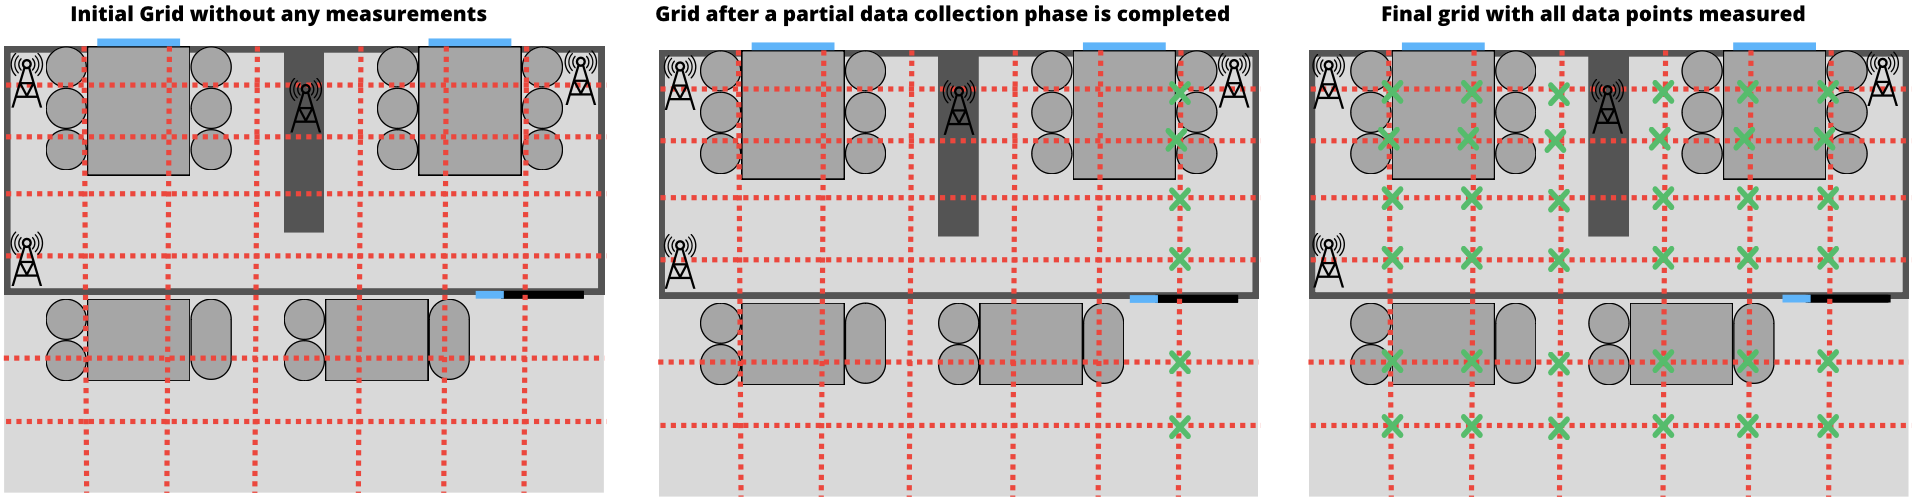
\includegraphics[width=\textwidth]{images/experiment_map_creation.png}
    \caption{A sketch of the meeting room partitioned into a grid decorated with beacon placements (red antenna) and measurement locations (circles with letters). The figure how the measurements are collected systematically in the meeting room.}
    \label{fig:experiment_map_creation}
\end{figure}
Whenever the collector stops at one of the collection points depicted in Figure \ref{fig:room_partition_measurements}, they press a button in the app, as depicted in Figure~\ref{fig:collecting_data}. This initiates data collection after five seconds, allowing the collector to position the device properly.
The phone provides auditory feedback when it has collected enough measurements and has reached a low enough standard deviation.
After successfully collecting data for the given grid point, the collector moves on to the next point.
Figure \ref{fig:experiment_map_creation} depicts a possible traversal, starting in the lower right corner of the grid. 


